%!TEX root = ../thesis.tex
%*******************************************************************************
%****************************** Second Chapter *********************************
%*******************************************************************************

\chapter{The LHC and the CMS experiment}
\label{sec:det}

\section{The Large Hadron Collider}
\label{det:LHC}

The LHC, situated at CERN in the Geneva area, is a circular hadron accelerator with a circumference of $27 \; \mathrm{km}$ that is designed for a collision energy of $\sqrt{s} = 14 \; \TeV$ \cite{1748-0221-3-08-S08001}.
This analysis uses data of proton-proton collisions taken in 2016 where the LHC reached a center of mass energy of $\sqrt{s}= 13 \; \TeV$.
The protons are assembled in bunches and accelerated to an energy of  $450 \; \GeV$ by various pre-accelerators before being injected into the LHC.
The two beams in the LHC run in opposite directions and are kept on their path by 2136 superconducting dipole magnets.

Collisions are induced at four points along the ring of the LHC, as shown in Figure \ref{fig:det_LHC}. The four main experiments are situated at these interaction points.
The ALICE (A Large Ion Collider Experiment) experiment is designed for heavy ion collisions resulting in events with a very high track multiplicity.
LHCb (Large Hadron Collider beauty) is focused on heavy flavor physics.
The two multi purpose experiments ATLAS (A Toroidal LHC Apparatus) and CMS (Compact Muon Solenoid) are designed to measure and search for low cross section processes.

\begin{figure}[htbp!]
  \begin{center}
      \resizebox{0.62 \textwidth}{!}{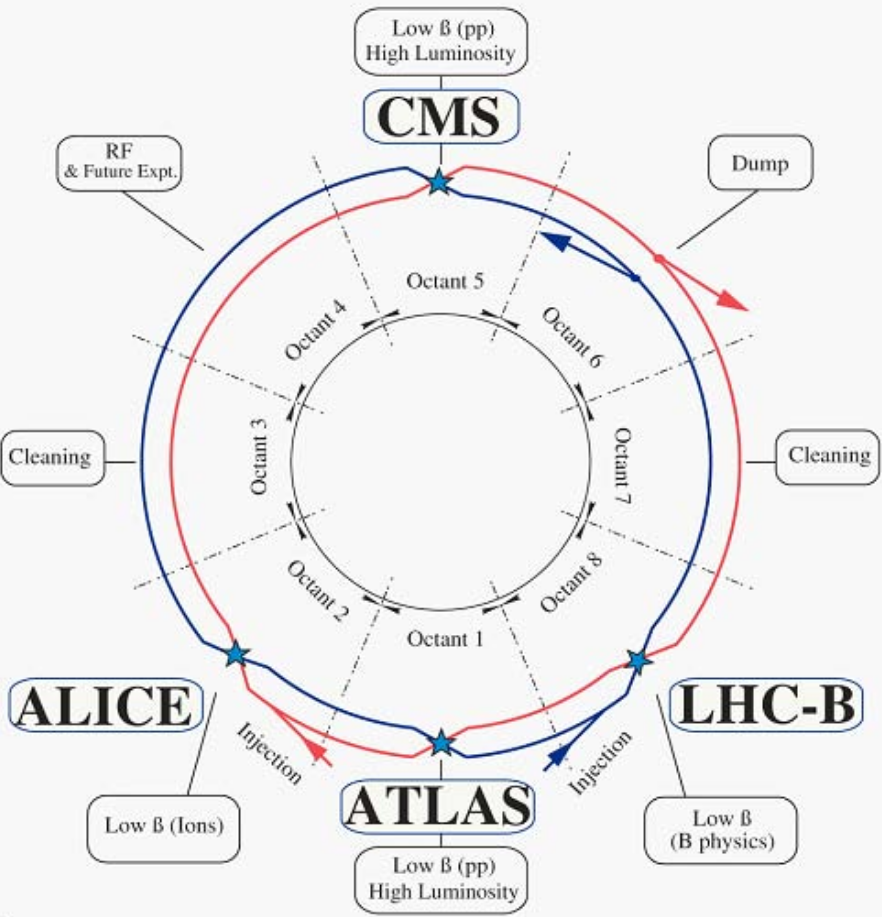
\includegraphics{Detector/Figures/LHC.png}}

\caption{Schematic of the LHC ring showing the two beams as well as the four major experiments. It also shows the injection points as well as the cleaning point and the beam dump. \cite{1748-0221-3-08-S08001}
  \label{fig:det_LHC}}
  \end{center}
\end{figure}

The instantaneous luminosity $\mathcal{L}$ is a measure for the rate of pp collisions.
It is related to the rate of events $\dot N$ of a process $k$ through the cross section $\sigma_k$:

\begin{equation}
\dot N_k = \mathcal{L} \cdot \sigma_k.
\end{equation}

The luminosity itself can be calculated from the beam properties:.

\begin{equation}
\mathcal{L} = \frac{N_b \cdot N_p^2 \cdot v}{\Sigma_x \Sigma_y}.
\end{equation}

Here, $N_b$ stands for the number of bunches, $N_p$ for the number of protons per bunch and $v$ for the rotation frequency of the LHC.
$\Sigma_x$ and $\Sigma_y$ are the effective widths of the overlap of the two beam profiles in x or y direction respectively. The luminosity is determined by measuring those beam profiles.
Special LHC conditions are used to calibrate the relevant parts of the detector for this measurement of the beam profiles. In a Van-der-Meer scan \cite{Zanetti:1357856} the two beams are shifted against each other, which allows to calibrate the detector for known configurations of $\Sigma_x,y$.
The calibrated detectors are then used to determine the instantaneous luminosity during data taking. 

In this analysis the data corresponds to an integrated luminosity of \lumivwunc taken at a center of mass energy of $\sqrt{s} = 13 \TeV$.

\section{The CMS detector}

The CMS experiments detector is a multi purpose detector for the study of particles from proton-proton, proton-lead and lead-lead collisions.
With a length of $21.6 \;\si{\meter}$ and a  diameter of $15 \;\si{\meter}$ it is relatively small and dense for its weight of 14000 tons \cite{Bayatian:922757}, thus the name 'compact'.

The detector is built of multiple radial layers ("onion structure") and split into a barrel region in the middle and two endcaps closing the detector structure as shown in the overview in Figure \ref{fig:det_CMS}.
The innermost part of the detector is the tracker, followed by the electromagnetic and then the hadronic calorimeter.
These parts of the detector are surrounded by the superconducting solenoid. The muon system is the last part of the detector and is situated outside the solenoid. It is interleaved with the iron return yoke of the magnet.

\begin{figure}[htbp!]
  \begin{center}
      \resizebox{0.89 \textwidth}{!}{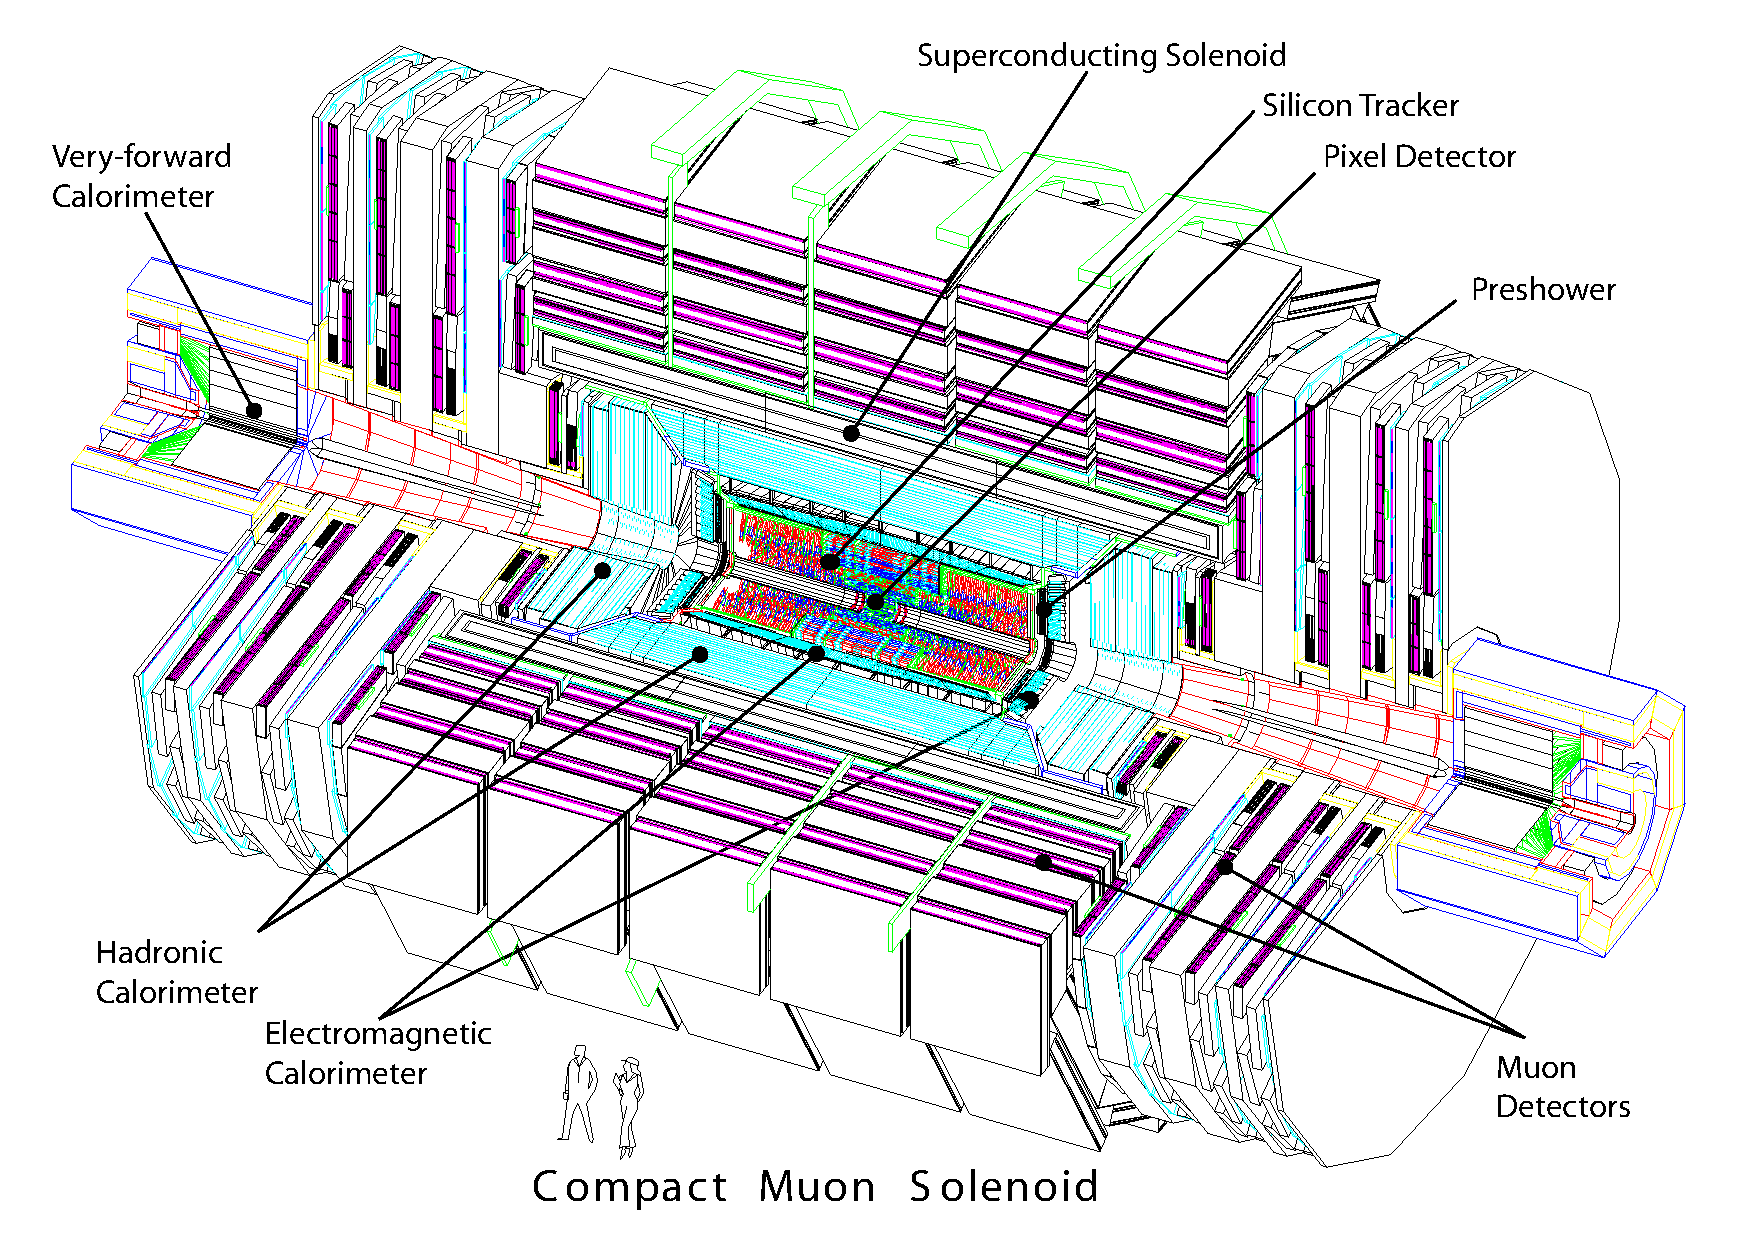
\includegraphics{Detector/Figures/cms_complete_labelled}}

\caption{The CMS detector and its relevant subsystems. \cite{Collaboration:1433717}
  \label{fig:det_CMS}}
  \end{center}
\end{figure}


The solenoid provides a magnetic field of $3.8 \;\si{\tesla}$ for the inner part of the detector (the tracker and calorimeters) and a field of about $2 \;\si{\tesla}$ in the muon system.
A total energy of $2.6 \;\si{\giga \joule}$ is stored in 2168 loops of superconducting cables.
This strong magnetic field leads to strongly bent tracks for charged particles, allowing a precise measurement of their momenta. 
The tracks of particles outside the magnet are bent in the opposite direction of those in the inner part.

The detector is described in a right-handed coordinate system with the origin in the interaction point.
The z-axis points in the direction of the counterclockwise beam, the y-axis points vertically upwards and the x-axis radially points towards the center of the LHC ring.
The $\varphi$ angle is defined in the x-y plane, while the angle $\theta$ is defined in the y-z plane. Instead of $\theta$ the pseudorapidity $\eta$ is used, since it is invariant under Lorentz transformation as long
as the momentum of a particle is large compared to its mass ($|\vec{\mathrm{p}}|\gg \mathrm{m}$):

\begin{equation}
\eta = -\ln{\tan{\frac{\theta}{2}}}.
\end{equation}

The subsequent sections describe the different parts of the detector including the triggering system that is used to select the collisions for which the data is stored for offline analysis.


\subsection{The tracking system}
\label{set:det_tracker}

The tracking system \cite{Bayatian:922757} is designed to measure both tracks and vertices with the highest possible precision.
This requires high granularity and, in the LHC environment, a fast response.

The tracking system is comprised of two parts: the inner one with pixels, the outer one with strips.
Its structure in the barrel as well as the endcaps is shown in Figure \ref{fig:det_Tracker}.

\begin{figure}[htbp!]
  \begin{center}
      \resizebox{0.75 \textwidth}{!}{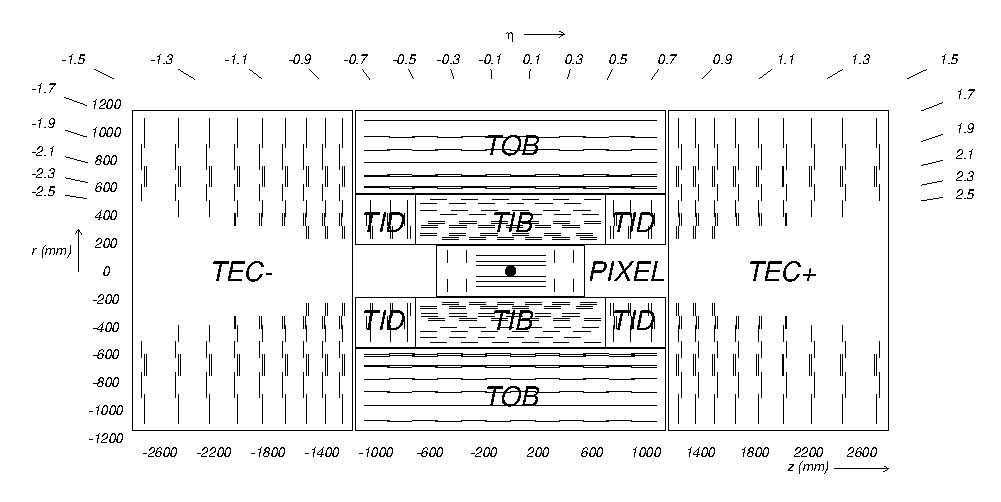
\includegraphics{Detector/Figures/TrackerLayout}}

\caption{The tracking system of the CMS detector in the barrel and endcap regions. The sketch shows the pixel as well as the strip tracker. The strip tracker consists of the inner barrel (TIB), outer barrel (TOB), inner disks (TID) and endcaps (TEC) parts \cite{Dominguez:1481838}.
  \label{fig:det_Tracker}}
  \end{center}
\end{figure}



The first pixel layer is located at a radius of $4.4 \;\si{\centi \meter}$ in the barrel and at $34.5 \;\si{\centi \meter}$ in the endcaps.
Both parts cover a range of $|\eta| < 2.5$.
The barrel region includes three layers of pixel detectors and ten layers of strip detectors, while the endcap includes two layers of pixels and twelve layers of strips.
The 66 million pixels measure $150 \times 100 \; \si{\micro \meter}$. The 9.6 million strips have a width of $80-180  \;\si{\micro \meter}$, together with the pixel that allows to separate even closely spaced
particle trajectories.
The position of each tracker part is precisely known from alignment analyses using tracks from collision events and cosmic muons \cite{Chatrchyan:2014wfa}.

The momenta of charged hadrons with a $\pt < 20 \GeV$ are measured with a resolution of $1\%$ at an incidence of ninety degrees \cite{Sirunyan:2017ulk}. The relative resolution decreases for higher \pt, reaching a resolution corresponding to 
the energy resolution of the calorimeter at several hundred \GeV. 
At low \pt, the resolution is dominated by multiple scattering of the particle in the tracker material \cite{1748-0221-9-10-P10009}. At high \pt, the resolution decreases as the bent of the track is
reduced making the \pt determination more difficult. The resolution in \pt is shown in Figure \ref{fig:det_trackeffs} for muons and charged pions.
Since high \pt partons usually produce multiple charged hadrons of lower \pt through fragmentation, the tracker can still contribute significantly 
to the measurement of high \pt jets.

\begin{figure}[htbp!]
  \begin{center}
      \resizebox{0.49 \textwidth}{!}{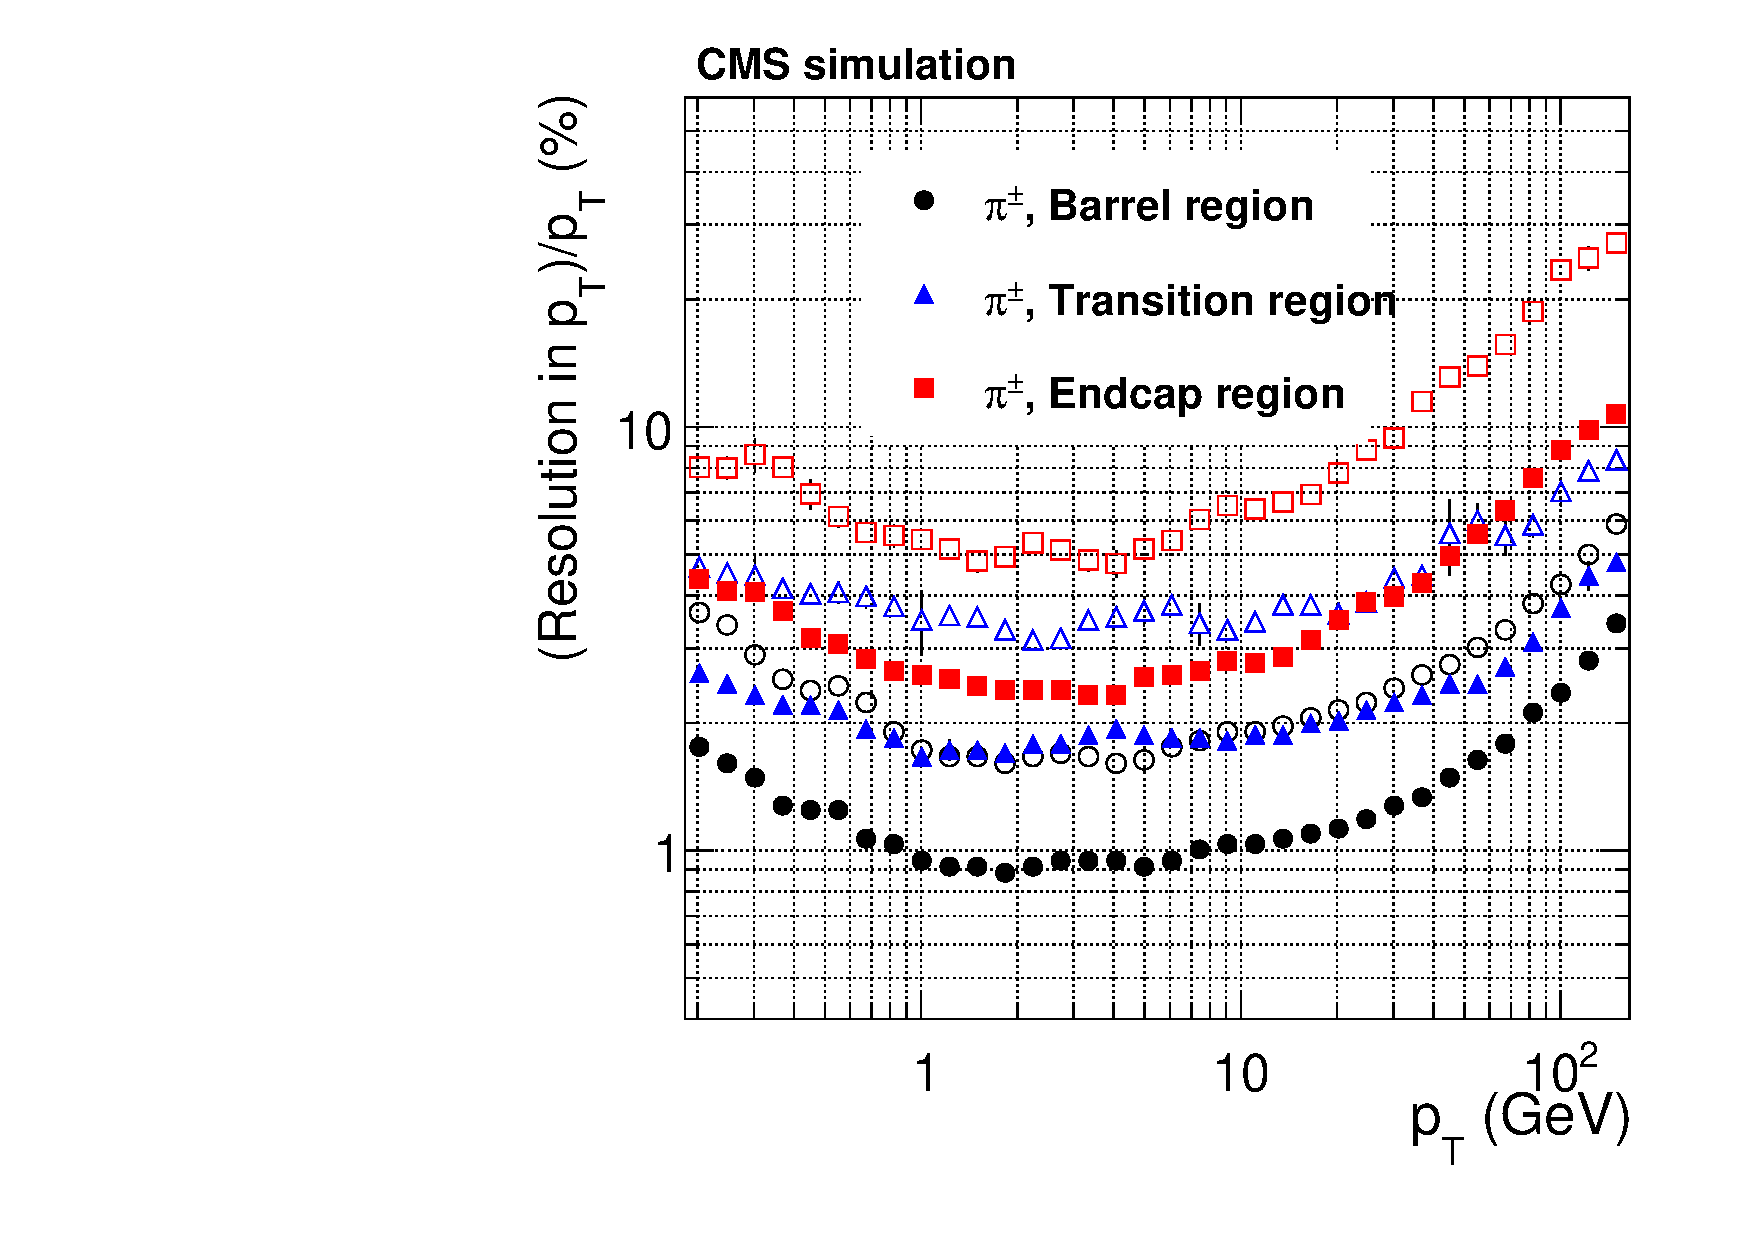
\includegraphics{Detector/Figures/trackpipt}}
      \resizebox{0.49 \textwidth}{!}{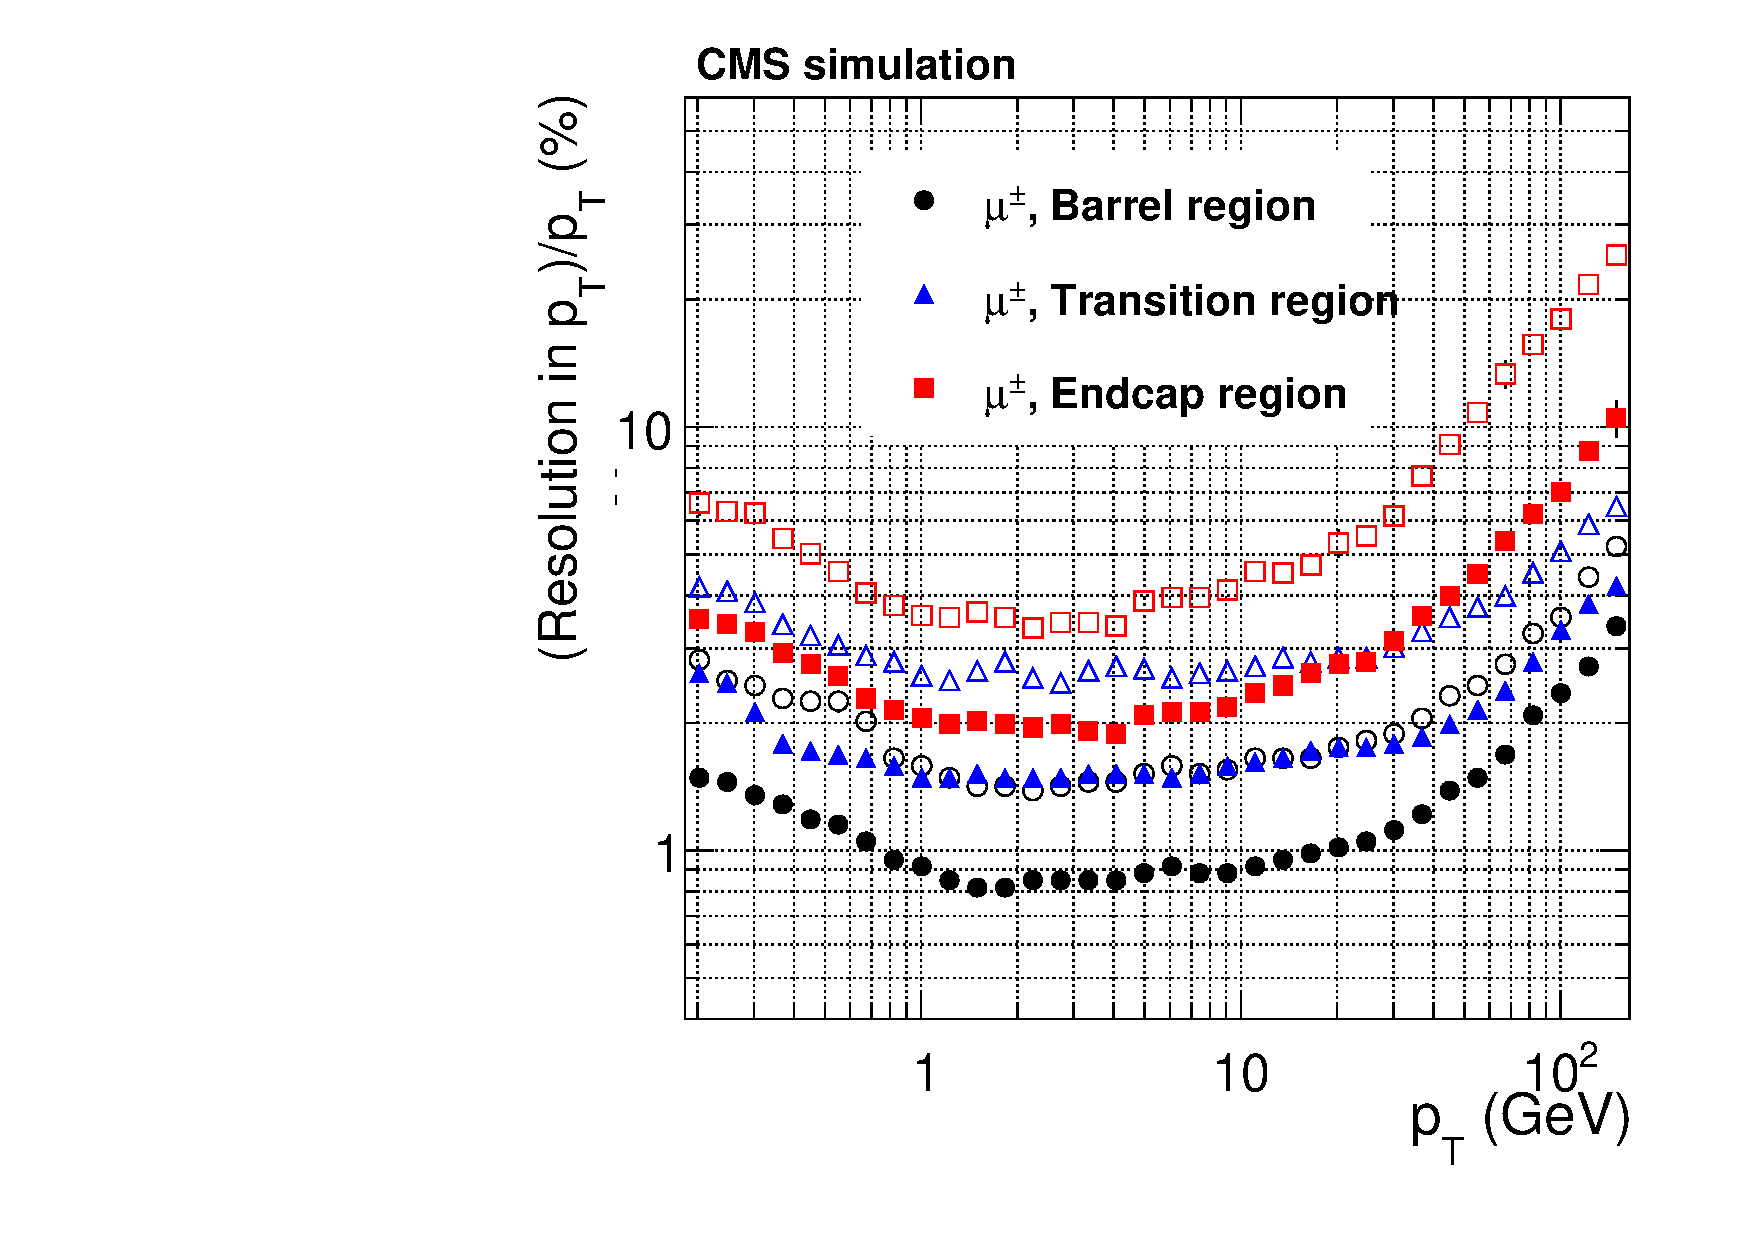
\includegraphics{Detector/Figures/trackmupt}}

\caption{Track \pt resolution depending on the track \pt for simulated charged pions (left) and muons (right). \cite{1748-0221-9-10-P10009}.
  \label{fig:det_trackeffs}}
  \end{center}
\end{figure}


\subsection{The electromagnetic calorimeter}

The electromagnetic calorimeter (ECAL)\cite{Bayatian:922757} measures the energy of electrons and photons that produce showers in the ECAL.
These electromagnetic showers should be contained within the ECAL. Additionally, the high granularity of the ECAL helps separate the signals from different particles.
A sketch of the structure of the ECAL is shown in Figure \ref{fig:det_ECAL}.

\begin{figure}[htbp!]
  \begin{center}
      \resizebox{0.75 \textwidth}{!}{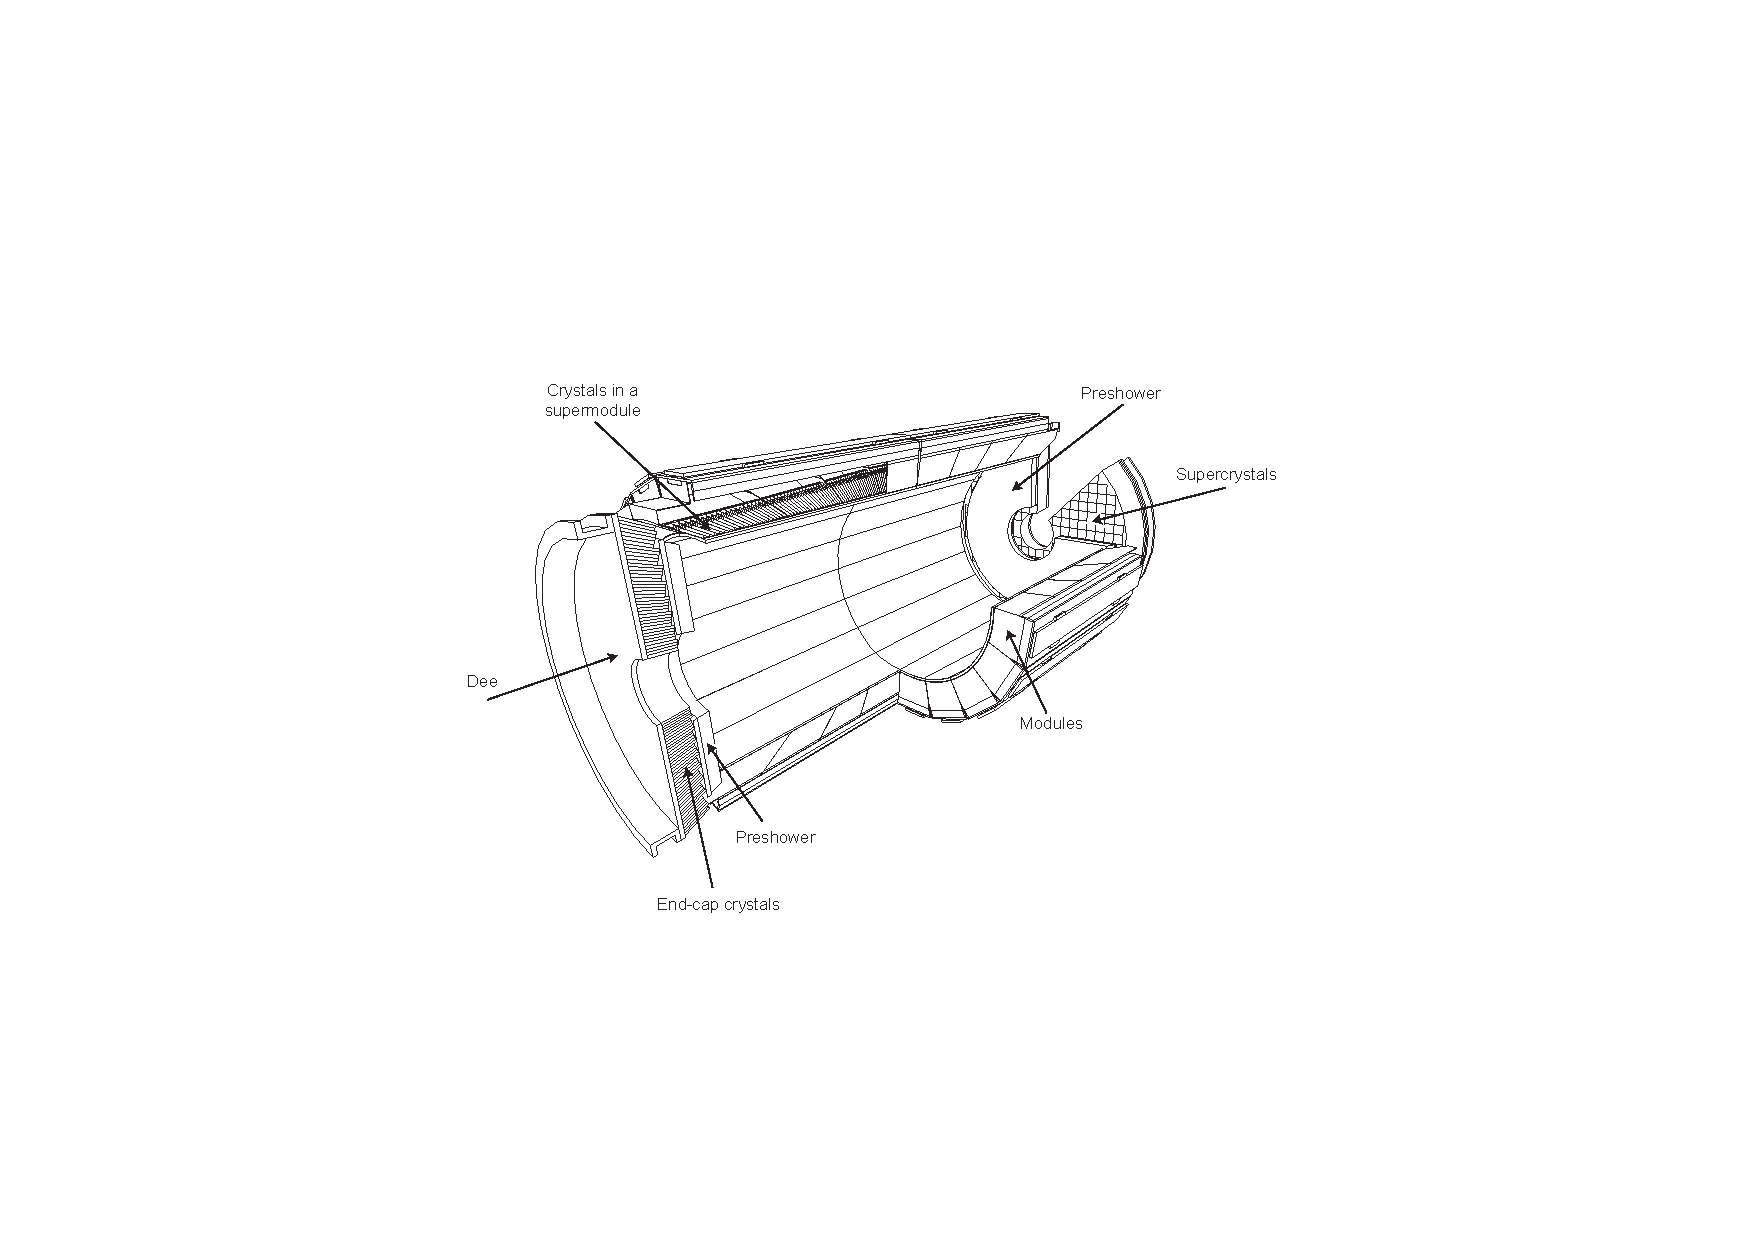
\includegraphics{Detector/Figures/ECAL}}

\caption{A sketch of the electromagnetic calorimeter showing the structure in the barrel and the endcaps as well as the preshower detectors. \cite{Chatrchyan:2009qm}.
  \label{fig:det_ECAL}}
  \end{center}
\end{figure}

The ECAL is made of lead tungstate with the barrel region covering about $|\eta| < 1.5$ and the endcaps covering $1.5 < |\eta|<3.0$. The crystals are $23 (22)  \;\si{\centi \meter}$ in the barrel (endcap) corresponding to about 26(25) radiation lengths.
For electrons and photons up to an energy of $1 \TeV$, more than $98  \%$ of the energy of each particle is completely contained in the ECAL.
The crystal depth also corresponds to roughly one interaction length. This implies that approximately two thirds of the hadrons start their shower in the ECAL.

The front of the crystals has a size of $2.2 \times 2.2 \;\si{\centi \meter \squared}$ in the barrel and $2.2 \times 2.2 \;\si{\centi \meter \squared}$ in the endcaps. This size corresponds to the Moliere radius of the 
lead tungstate of $2.2 \;\si{\centi \meter}$.
The electronic noise in the ECAL is measured to be about $40 \MeV$ per crystal in the barrel and about $100 \MeV$ in the endcaps.

The energy resolution for an electron measured in the ECAL can be parameterized depending on the electron energy as follows \cite{Sirunyan:2017ulk}:

\begin{equation}
\frac{\sigma}{\mathrm{E}} = \frac{2.8\%}{\sqrt{\mathrm{E}/\GeV}} \oplus \frac{12\%}{\mathrm{E} / \GeV} \oplus 0.3\%.
\end{equation}

The first term represents a stochastic term caused by fluctuations such as the amount of intrinsic variations of the showering itself. The second term is caused by noise from the electronics and the constant third term is related
to calibration uncertainties, detector non-uniformity and radiation damage.

Photons in jets have a typical energy range of $1-50 \GeV$ where the resolution of the ECAL is excellent.

The so-called preshower detector is situated in front of the two ECAL disks in the endcaps.
The preshower contains two layers: The first is a lead radiator followed by silicon strip sensors.
The detector has a much higher granularity than the ECAL, which allows measuring the initial position of a shower from an electron or photon with a high precision.
The purpose of the preshower is to discriminate  between neutral pions decaying into two photons and prompt single photons.
Additionally, a coincidence between ECAL and preshower can be used to identify electrons and photons.
The performance of the preshower is degraded through a large number of neutral pions resulting from hadrons interacting with the tracker material.

\subsection{The hadronic calorimeter}

The hadronic calorimeter (HCAL)\cite{Bayatian:922757} is a sampling calorimeter consisting of layers of brass absorbers and plastic scintillators.
Its purpose is to measure the energy of hadronic showers with a high precision. Additionally, it prevents the hadronic showers from leaking into the muon system.
In the barrel it covers a range of $|\eta|< 1.3$ with a corresponding endcap coverage of $1.3 <|\eta|< 3.0$.
In the barrel it is about six interaction lengths thick at normal incidence, increasing to over ten interaction lengths at lower incidence angles.
The whole HCAL is shown as a sketch in Figure \ref{fig:det_HCAL}.



\begin{figure}[htbp!]
  \begin{center}
      \resizebox{0.75 \textwidth}{!}{\includegraphics{Detector/Figures/hcaldisplay.eps}}

\caption{A quarterly schematic of the hadronic calorimeter showing the HCAL in the barrel(HB) and the endcaps(HE), the outer HCAL (HO) and the forward HCAL (HF)  \cite{2010JInst...5T3014C}.
  \label{fig:det_HCAL}}
  \end{center}
\end{figure}



The outer hadronic calorimeter (HO) is situated outside the solenoid coil, increasing the interaction length as an additional absorber.
In the very central region, the interaction length is further increased by additional layers of steel.
Including the ECAL, the total calorimeter system has a thickness corresponding to a minimum of about twelve interaction lengths in the barrel and ten interaction lengths in the endcaps.
The individual towers of the ECAL have a cross section of $\Delta \eta \times \Delta \varphi = 0.087 \times 0.087$ in the central region of $|\eta|< 1.6$ and a cross section of $\Delta \eta \times \Delta \varphi = 0.017 \times 0.017$
in the more forward region \cite{Bayatian:922757}.

The electronic noise is measured to be about $200 \MeV$ per tower \cite{Sirunyan:2017ulk}.
The combined energy resolution for ECAL and HCAL has been measured with a pion beam to be 

\begin{equation}
\frac{\sigma}{\mathrm{E}} = \frac{110\%}{\sqrt{\mathrm{E}/\GeV}} \oplus 9\%.
\end{equation}

The two parts of the hadron forward calorimeter (HF) are positioned in the very forward(backward) region of the detector at a distance of $11 \; \si{\meter}$ from the interaction point.
It covers a region of up to $|\eta| \approx 5$. It consists of steel absorbers and quartz fibers of two different lengths. The long quartz fibers correspond to roughly ten interaction lengths. The difference in the signal from the short and the long fibers is used to estimate the hadronic and electromagnetic components of the shower.

\subsection{The muon system}

High energy muons mostly interact with matter through ionization.
They are generally neither stopped by nor decay within the detector, so the momentum can only be measured by reconstructing their tracks.

The purpose of the muon system as the outermost part of the detector is to identify muons and measure their momentum.

The muon system \cite{Bayatian:922757} consists of four layers with three steel layers of the return yoke of the solenoid between them.
The central region is covered by Drift Tubes (DT) in the region of $|\eta|< 1.2$. The outer region is covered by Cathode Strip Chambers (CSC) in the region of $0.9<|\eta|<2.4$.
Additionally, Resistive Plate Chambers (RPC) cover the range of $|\eta|<1.6$.
A sketch of the whole muon system is shown in Figure \ref{fig:det_muon}.

\begin{figure}[htbp!]
  \begin{center}
      \resizebox{0.75 \textwidth}{!}{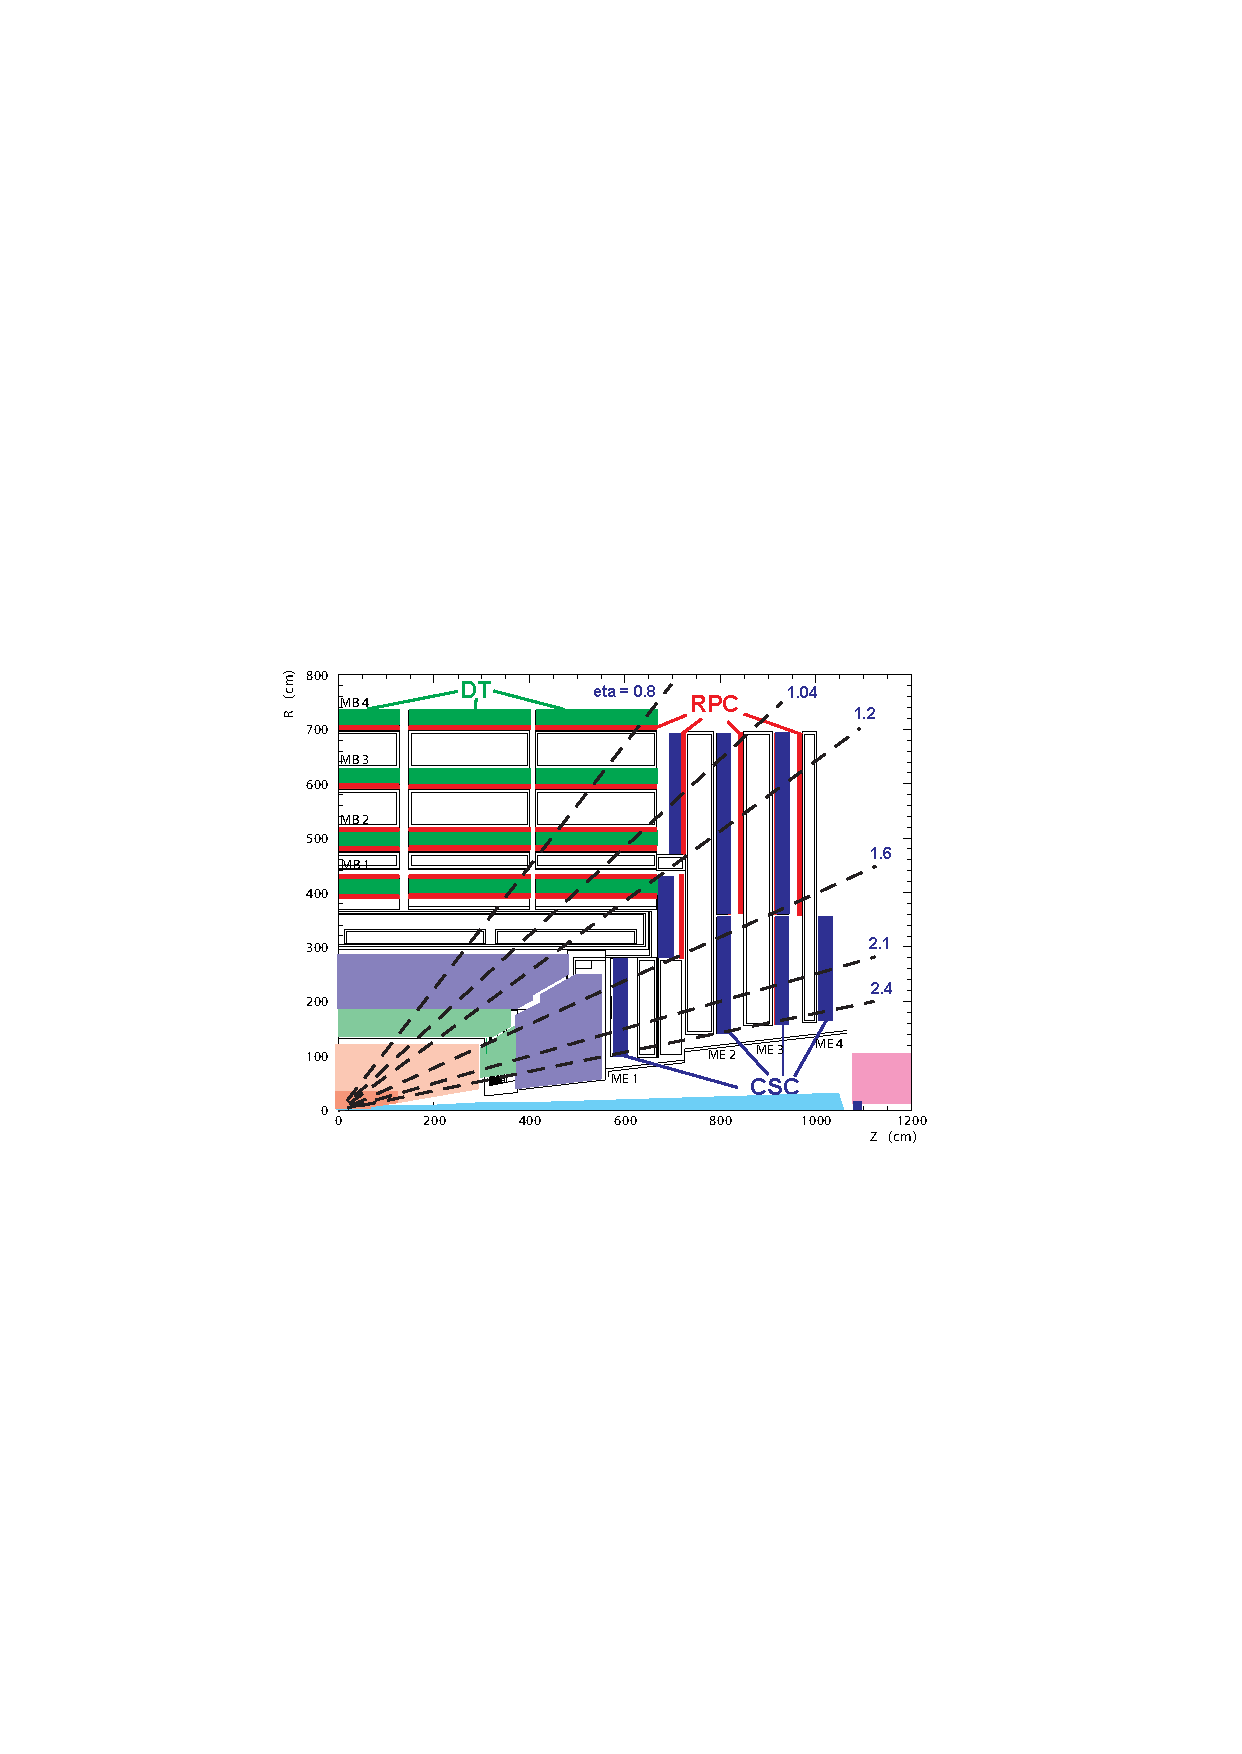
\includegraphics{Detector/Figures/Muon}}

\caption{A quarterly schematic of the muon system showing the Drift Tubes(DT) in the central part, the Cathode Strip Chambers(CSC) in the outer part and the Resistive Plate Chambers(RPC). \cite{Bayatian:922757}.
  \label{fig:det_muon}}
  \end{center}
\end{figure}

The DT chambers are filled with a mixture of argon and carbon dioxide. The chambers themselves contain layers which are rotated against each other,
which allows measuring both the $\varphi$ and the $\eta$ projection of the track. The DTs are also used for triggering.

The CSCs are positioned at a right angle with respect to the DTs. The single chambers consist of six gas gaps each. The two coordinates of the track are determined by radial cathode strips and perpendicular anode wires.
The spatial resolution of both the CSCs and the DTs is in the range of $100-200 \; \si{\micro \meter}$, depending on $\eta$.

The RPC system consists of 480 chambers. Their very high time resolution in the sub nano second range allows them to be used for triggering and the association of single muon tracks with a specific bunch crossing.

\subsection{Triggering}
\label{set:det_trigger}

The LHC delivers a collision rate of $40 \;\si{\mega \hertz}$. In order to record the data as it is measured by the detector, this data volume has to be reduced to a manageable size by
only keeping those events for further study in which a relevant result is observed. A two-tiered triggering system is used to reduce the final rate of events to $100 \;\si{\hertz}$.
First the hardware-based Level-1 (L1) Trigger is used to reduce the number of events for the software-based high-level trigger (HLT) \cite{Bayatyan:706847,Tapper:2013yva}.

The L1 trigger consists of programmable electronics using information from the calorimeters as well as the muon system as shown in Figure \ref{fig:det_Trigger}. The L1 trigger is separated into the muon trigger and the calorimeter trigger. The tracking system is not used at this stage of triggering.
 The muon trigger combines track information from the CSCs, DTs and RPCs. It uses information from the calorimeters for the isolation of the muons.
The calorimeter trigger combines the ECAL, HCAL and HF. Besides muon triggers, algorithms targeting electrons/photons, taus, jets and the overall energy deposition in the detector are used. Requiring a muon to be contained within a jet allows to target jets originating from a b quark where the B-hadron decays further into a final state containing a muon.
The L1 trigger has a maximal latency of $3.8  \;\si{\micro \second}$ in which a trigger decision has to be delivered to the HLT.

\begin{figure}[htbp!]
  \begin{center}
      \resizebox{0.75 \textwidth}{!}{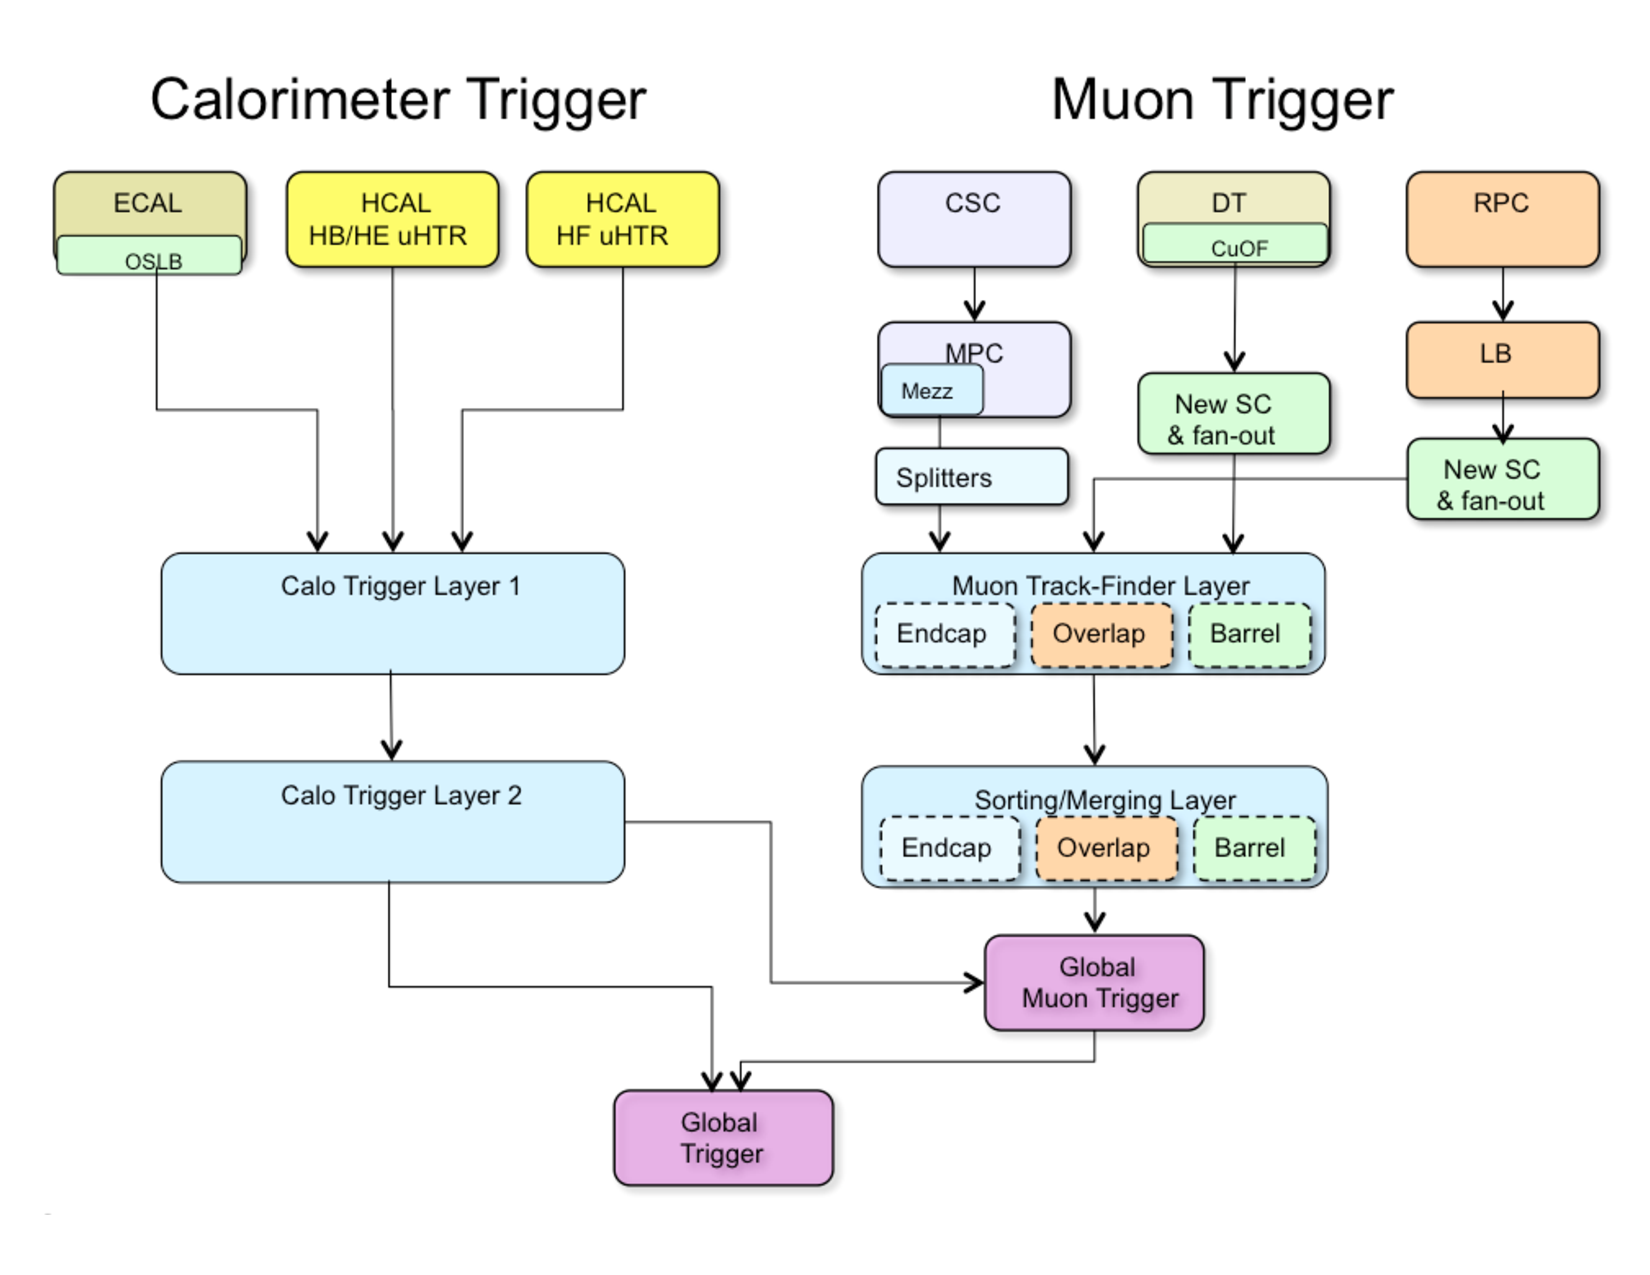
\includegraphics{Detector/Figures/Trigger}}

\caption{ Dataflow of the L1 trigger system showing the combination of information from the different subsystems \cite{Tapper:2013yva}.
  \label{fig:det_Trigger}}
  \end{center}
\end{figure}

The HLT is the second step of the triggering system. It reduces the number of events from $100 \; \si{\kilo \hertz}$ to $100 \; \si{\hertz}$.
Compared to the L1 trigger, it uses more sophisticated reconstruction techniques, which are generally close to the final reconstruction that is used for analysis.
The HLT starts from the L1 decision. It then combines information from the complete detector, including tracks, to reconstruct the respective particle in the path.
Finally, further thresholds on the kinematics, the isolation or the reconstruction quality are required. 
These steps are performed sequentially. If one step fails the sequence is stopped. 

In order to be able to reduce the rate of certain trigger paths for both the L1 and the HLT, some trigger paths only consider a fraction of events. This technique is called prescaling. If a trigger path is prescaled by two it only considers every second event.

A detailed study of the lepton triggers which are used in this analysis is presented in Chapter \ref{sec:Trigger}. The measurement of the trigger efficiency is 
discussed as well.

